\documentclass[11pt]{article}
\usepackage[margin=0.85in]{geometry}
\usepackage{amsmath,amssymb,graphicx,xurl,hyperref}
\setlength{\parindent}{0pt}\setlength{\parskip}{7pt}
\begin{document}
{\LARGE Actual chart units and the algorithm obligation}\par
November9,2026. Source \texttt{7bb276623}. Unsigned producer evidence
throughout [pcc:unverified].

\textbf{New actual-object result.} The rational denominator and earlier scalar
normalizer evaluate to units at every interpolation value in every commutative
coefficient target where the image of two is nilpotent. This includes every
$\mathbb Z/(2^p)$ value and permits further nilpotents/zero divisors. A constructed
normalized finite entry differs from the old scalar-square entry by one actual
common unit, preserving every scalar divisibility threshold.

\textbf{Chart proof.} Write $\mathcal O$ for the actual rational integral ring
and $\alpha=2^{a+1}$. Actual nonzero differences satisfy $|m-j|<\alpha$, hence
$v_2(m-j)\leq a$. Therefore $\alpha/(m-j)$ is even in $\mathcal O$; the
zero equal-index ratio is even too. In the already constructed puncture chart,
\[
 B_s(t_m+\alpha z)=\rho_m
  \begin{cases}1&s=m\\ \alpha z/(m-s)&s\ne m\end{cases}
  \prod_{j\ne m,s}(1+\alpha z/(m-j)).
\]
Under any coefficient map killing two, this polynomial is constant $\rho_m$
when $s=m$ and zero otherwise. Consequently the actual polynomials satisfy
\[
 D=\sum_s B_s\equiv\rho_m\pmod2,\qquad
 R=\sum_s\rho_s^{-2}B_s\equiv\rho_m^{-1}\pmod2.
\]
The old normalizer's actual rational formula is connected to this integral
polynomial. Its definition is exposed for the module API, without changing
its value or any previous proof body.

\textbf{Units after substitution.} The actual residue kernel proves
$D-C(\rho_m)$ and $R-C(\rho_m^{-1})$ divisible by $C(2)$. Evaluation under
$\pi:\mathcal O\to A$ gives a unit plus $\pi(2)$ times a value. If $\pi(2)$
is nilpotent, the perturbation is nilpotent, so the sum is a unit for every
$z\in A$. No assumed unit for an unspecified normalizer is used.
\newpage
{\Large Finite comparison and verification}\par
Let $n_s$ be the actual base-chart evaluation and $d$ the unit produced for
$D$. Define $U_s=d^{-1}n_s^2$. If $r$ is the actual old-normalizer evaluation,
then $c=rd$ is a unit and
\[
 cU_s=rn_s^2,\qquad e\mid rn_s^2\iff e\mid U_s.
\]
This does not prove a minimal Smith/Newton factorization, an optimal mode count
or a full recursive cost. Historical panel rows remain unchanged and are not
relabelled as new rational-kernel measurements.

\begin{center}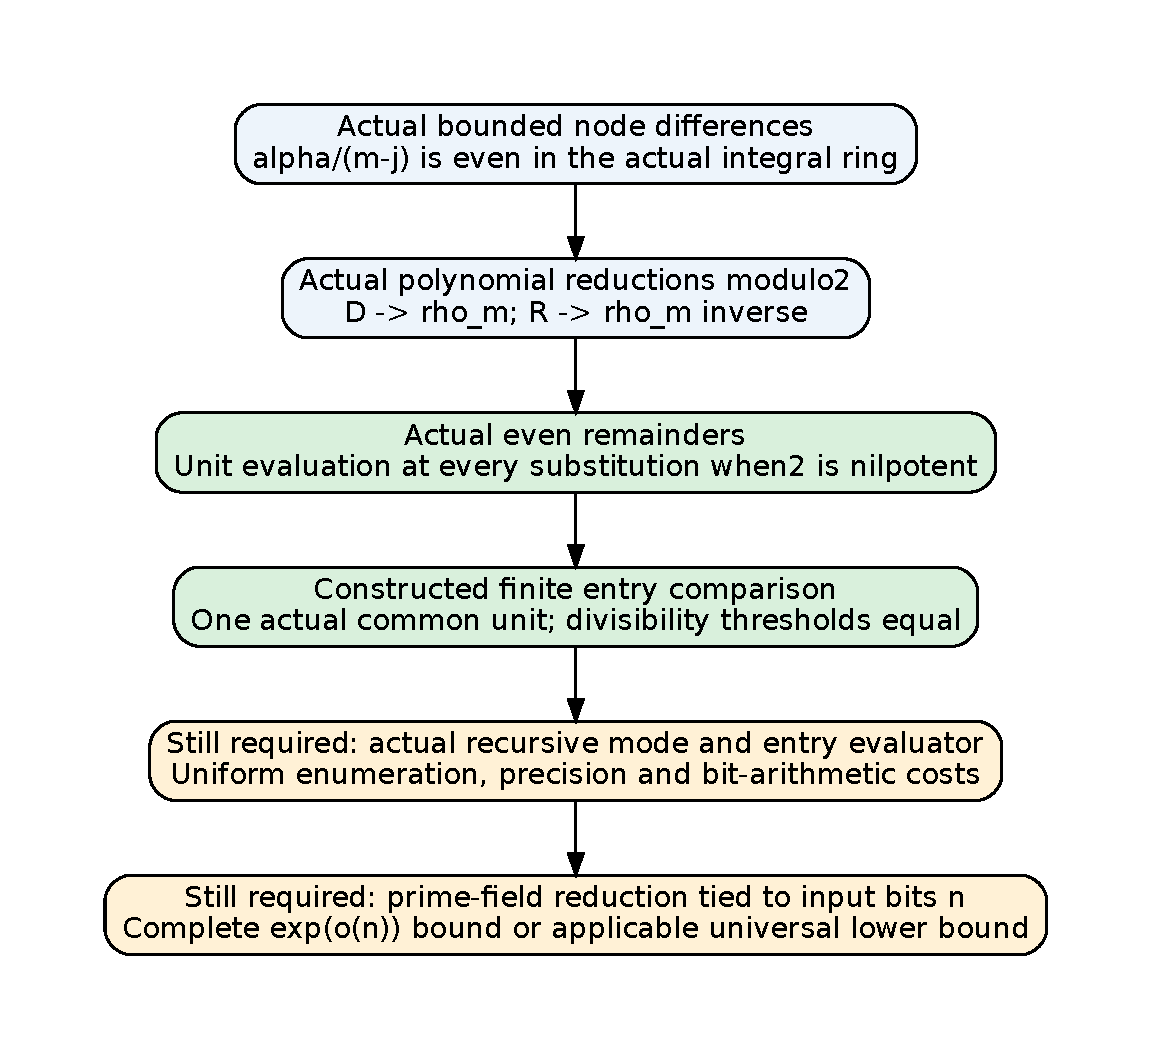
\includegraphics[width=0.96\linewidth,height=0.53\textheight,keepaspectratio]{bridge.pdf}\end{center}

Nine unsigned PCC bindings (prefix \texttt{PCC-20261109-}): even ratio777347,
denominator reduction9c4c4f, old-normalizer evaluation65b9f5, normalizer
reduction53504f, denominator units485e5c, normalizer units7cea35, modular
comparison units c9a342, finite entry identity51ff85, divisibility ff3e71.
Canonical hashes and successful/failed logs are retained under \texttt{lean/}.
Actual source audit and fresh import-inclusive status are appended to the
companion report after completion. No new native census was run.
\newpage
{\Large Goal assessment and exact remaining dependency}\par
The requested faithful Lean proof of existence or nonexistence of a novel
classical sub-exponential algorithm for general prime-field ECDLP is still
absent. The unresolved dependency is mathematical, not machine access.

\textbf{Existence route.} Actual clearing, finite recovery and this unit bridge
provide algebraic components. A complete program still needs an actual all-level
mode/child-entry evaluator, packing and input construction, success/recovery
proofs and every construction, precision, failed-attempt and bit-arithmetic cost.
Its reduction must connect network/circuit size $s$ to the ECDLP input length
$n$ and establish total $T(n)=\exp(o(n))$. Identifying $s$ with $n$ without a
proved reduction is insufficient. Supplied tensors or coefficient buffers do
not establish their own efficient construction.

\textbf{Representation alternative.} The scaled accumulator has a proved
scaled target congruence and valid cross-precision cancellation. Native canonical
extraction, coefficient delivery, retained-state and recomputation costs remain
separate. The closed native census supplies finite correctness, not asymptotic
cost evidence.

\textbf{Origin and jet alternatives.} A physical-coordinate transformation
need not act as a Boolean gauge; the prior finite counterexample remains.
A correction $W+C(T)H$ with $C(0)=0$ retains $W(0)$, although higher jets remain
adjustable. Neither fact rules out a different target-preserving channel or a
future all-level rank construction.

\textbf{Nonexistence route.} These family-specific facts are not a lower bound
for every non-generic algorithm. An algorithmic upper-bound envelope cannot
supply that lower bound. No applicable unrestricted lower-bound theorem is
established here. Assuming the desired runtime or correctness in a wrapper
would not constitute the requested proof.

\textbf{Sources.} Actual formal chart/residue modules and earlier reports;
pinned OpenAI Oct25,2026 manuscript D.4.3--D.4.7/D.9/D.10; primary Mathlib
PadicNorm and Nilpotent.Basic. KB unavailable. No priority or exhaustive-search
claim. Exact next obligations are in PLAN.md and the current goal-status note.
\end{document}
